\documentclass[11pt,letterpaper]{article}
\usepackage[utf8]{inputenc}
\usepackage[T1]{fontenc}
\usepackage{mathptmx}
\usepackage{courier}
\usepackage{xcolor}
\renewcommand{\figurename}{Figura}\renewcommand{\tablename}{Tabla}
\hyphenpenalty=10000\exhyphenpenalty=10000\emergencystretch=4em\tolerance=2000
\usepackage[margin=1.15in]{geometry}
\usepackage{graphicx,booktabs,float,enumitem,microtype}
\usepackage[font=small]{caption}
\usepackage[colorlinks=true,linkcolor=blue!60!black,urlcolor=blue!60!black,citecolor=blue!60!black]{hyperref}
\setlist{itemsep=2pt,topsep=4pt}
\renewcommand{\arraystretch}{1.1}
\newcommand{\code}[1]{\texttt{#1}}
\setlength{\parskip}{4pt}
\setlength{\parindent}{0pt}

\begin{document}

\begin{center}
\rule{\linewidth}{1.2pt}\\[8pt]
{\LARGE\bfseries Predicción del Rendimiento y Abandono Universitario\\[2pt] mediante Aprendizaje Automático}\\[8pt]
\rule{\linewidth}{0.6pt}\\[12pt]
{\bfseries Jaime Tuesta de Simón}\\
Universidad Pontificia Comillas (ICAI)\\[14pt]
\textbf{Abstract}\\[4pt]
\begin{minipage}{0.88\linewidth}
\small\hspace{1.2em}Este trabajo analiza el rendimiento y la retención de estudiantes universitarios mediante técnicas de aprendizaje automático aplicadas a un conjunto de datos real. Se abordan tres paradigmas: clasificación del resultado académico final (graduado, abandono o matriculado), regresión de la nota media del segundo semestre, y clustering no supervisado para descubrir perfiles de estudiantes. Los resultados muestran que el rendimiento académico es el predictor más potente: en regresión, las variables del primer semestre, junto con las de contexto, permiten estimar la nota del segundo con un $R^2 \approx 0{,}78$, y en clasificación la regresión logística alcanza un F1-macro $\approx 0{,}72$. Se discuten las implicaciones y las limitaciones de estos resultados para el seguimiento de estudiantes en riesgo de abandono.
\end{minipage}
\end{center}

\section{Análisis Exploratorio de Datos}

El dataset contiene información académica, socioeconómica y macroeconómica de 4.424 estudiantes universitarios, distribuida en 37 columnas: 19 numéricas y 18 categóricas (una de ellas es la variable objetivo). No se detectaron valores nulos ni duplicados.

La variable objetivo toma tres valores: \emph{Graduado} (49,93\,\%), \emph{Abandono} (32,12\,\%) y \emph{Matriculado} (17,95\,\%). Para preservar estas proporciones se utilizó una división estratificada del conjunto de datos, y el desbalanceo se compensó con \code{class\_weight='balanced'} en los modelos de clasificación que lo admiten.

\begin{figure}[!htb]
\centering
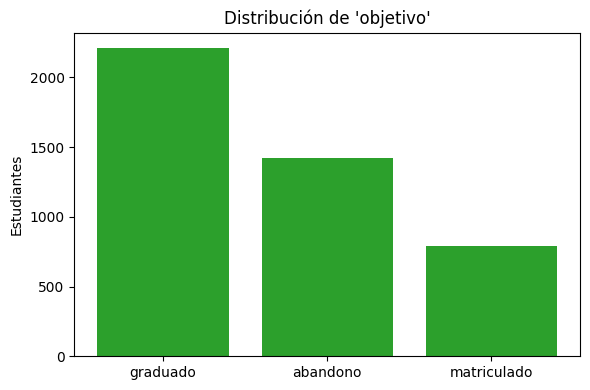
\includegraphics[width=0.5\linewidth]{figs/f1.png}
\caption{Distribución de la variable objetivo.}
\end{figure}

Entre las variables numéricas destacan el rendimiento académico en ambos semestres (asignaturas matriculadas, evaluadas, aprobadas y nota media), la nota de admisión, la edad al matricularse y variables macroeconómicas como la tasa de desempleo y el PIB. El mapa de correlaciones (Figura~\ref{fig:corr}) revela una fuerte relación entre las variables de primer y segundo semestre, lo que anticipa su relevancia predictiva.

\begin{figure}[!htb]
\centering
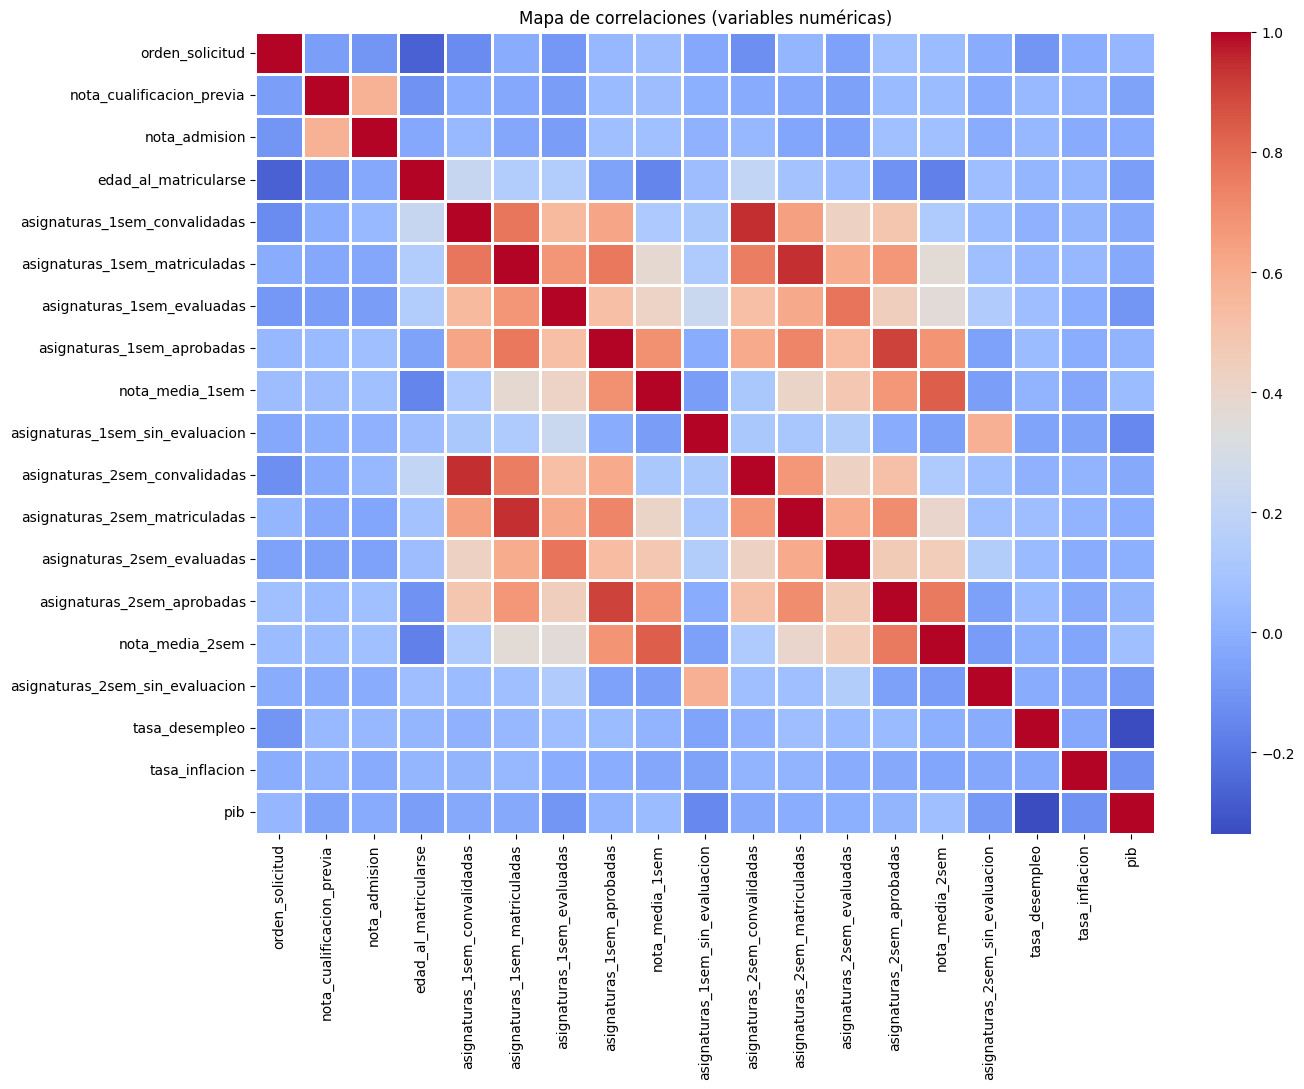
\includegraphics[width=0.72\linewidth]{figs/f2.png}
\caption{Mapa de calor de correlaciones entre variables numéricas.}\label{fig:corr}
\end{figure}

Las variables categóricas incluyen el modo de solicitud de ingreso, la nacionalidad, el curso, la cualificación previa, la ocupación y cualificación de los padres, y variables binarias como becado o matrícula al día.

\section{Preprocesado}

\paragraph{Limpieza y tratamiento de outliers.}
Se verificó la ausencia de valores nulos y filas duplicadas, confirmando que el dataset no requiere ningún tipo de imputación ni eliminación de registros. Se detectaron valores atípicos mediante el rango intercuartílico (IQR) en varias variables numéricas, siendo \code{nota\_media\_2sem} (877) y \code{nota\_media\_1sem} (726) las más afectadas. No se eliminaron, ya que pueden corresponder a situaciones reales extremas.

\paragraph{Exclusión de variables por data leakage.}
Para la tarea de regresión, cuyo objetivo es predecir la nota media del segundo semestre (\code{nota\_media\_2sem}), se excluyeron todas las variables relativas al segundo semestre, ya que no estarían disponibles en el momento de la predicción. También se excluyó la variable objetivo, por ser la etiqueta de la tarea de clasificación.

\paragraph{División train/test y transformación.}
El dataset se dividió en un 80\,\% para entrenamiento (3.539 instancias) y un 20\,\% para test (885 instancias). En clasificación, la división se realizó de forma estratificada para preservar la proporción de clases en ambos subconjuntos, obteniendo distribuciones prácticamente idénticas: Graduado $\approx$ 49,9\,\%, Abandono $\approx$ 32,1\,\% y Matriculado $\approx$ 17,9\,\%. Las transformaciones se aplicaron mediante un \code{ColumnTransformer} ajustado solo con el conjunto de entrenamiento para evitar data leakage:
\begin{itemize}
\item Variables numéricas (19 en clasificación; 13 en regresión): normalización con \code{StandardScaler} ($\mu=0$, $\sigma=1$).
\item Variables categóricas (17 en ambas tareas): codificación con \code{OneHotEncoder}, resultando en 241 características en clasificación y 240 en regresión.
\end{itemize}
La variable objetivo de clasificación se codificó con \code{LabelEncoder}. Los preprocesadores se serializaron con \code{joblib} para reutilizarlos en los notebooks de modelado sin necesidad de reejecutar este paso.

\section{Clasificación}

El objetivo de esta tarea es predecir la \textbf{situación final del estudiante} (\emph{Graduado, Abandono, Matriculado}) a partir de sus características académicas, socioeconómicas y demográficas. Se emplean todas las variables disponibles, incluidas las del segundo semestre. Se comparan tres modelos de diferente complejidad.

\paragraph{Modelos}
\begin{itemize}
\item \textbf{Logistic Regression}: clasificador lineal que modela la probabilidad de cada clase mediante una función sigmoide.
\item \textbf{Random Forest}: \emph{ensemble} de árboles de decisión entrenados en paralelo (\emph{bagging}). Captura relaciones no lineales y es robusto frente al ruido.
\item \textbf{Gradient Boosting}: \emph{ensemble} de árboles entrenados en secuencia (\emph{boosting}), donde cada árbol corrige los errores del anterior.
\end{itemize}

\paragraph{Resultados}
La métrica principal es el \textbf{Macro F1-score}, que pondera por igual todas las clases independientemente de su tamaño, penalizando especialmente los fallos en la clase minoritaria (\emph{Matriculado}).

\begin{table}[H]
\centering
\caption{Resultados de clasificación en el conjunto de test.}
\begin{tabular}{lccccc}
\toprule
Modelo & Accuracy & Macro F1 & F1 Abandono & F1 Graduado & F1 Matriculado\\
\midrule
Logistic Regression & 0,76 & 0,72 & 0,81 & 0,82 & 0,53\\
Random Forest & 0,78 & 0,68 & 0,79 & 0,86 & 0,40\\
Gradient Boosting & 0,77 & 0,69 & 0,79 & 0,86 & 0,42\\
\bottomrule
\end{tabular}
\end{table}

Pese a tener la menor accuracy, Logistic Regression obtiene el mejor Macro F1 (0,72), gracias a que su uso de \code{class\_weight='balanced'} le permite predecir mejor la clase Matriculado. Random Forest y Gradient Boosting obtienen resultados similares entre sí, con mayor accuracy pero peor rendimiento en la clase minoritaria, como confirman las matrices de confusión (Figura~\ref{fig:cm}).

\begin{figure}[!htb]
\centering
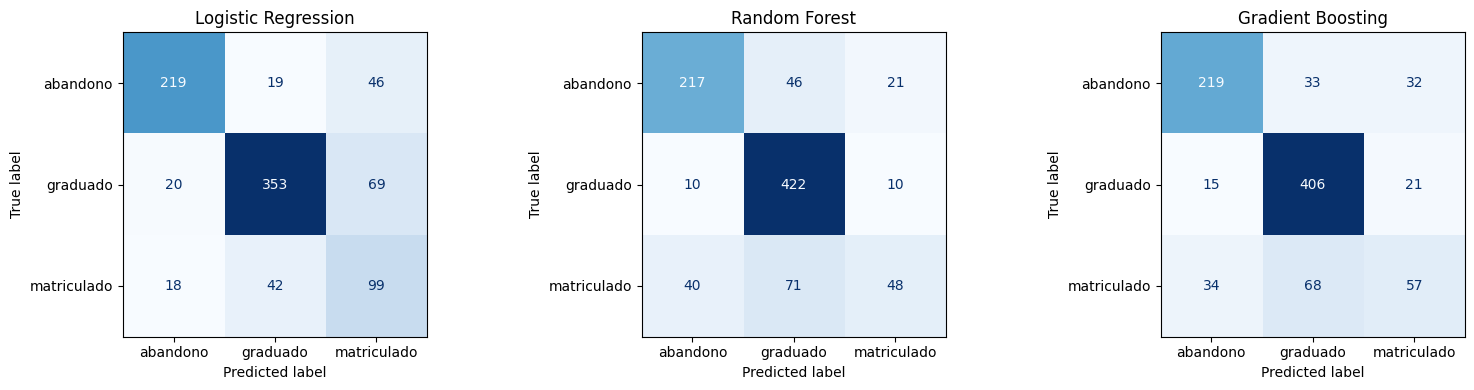
\includegraphics[width=\linewidth]{figs/f3.png}
\caption{Matrices de confusión de los tres modelos en el conjunto de test.}\label{fig:cm}
\end{figure}

\paragraph{Importancia de variables}
Las variables más determinantes en los tres modelos son las relacionadas con el número de asignaturas aprobadas. En concreto, \code{asignaturas\_2sem\_aprobadas} encabeza los tres rankings (con un peso especialmente alto en Gradient Boosting), seguida de las asignaturas aprobadas del primer semestre y de las notas medias de ambos semestres. Para Logistic Regression se calcula la Permutation Importance al no disponer de \code{feature\_importances\_} en el modelo. Dado que esta tarea incluye variables del segundo semestre, el modelo relaciona el rendimiento del primer año con el desenlace final; por sí solo no constituye un sistema de alerta temprana.

\section{Regresión}

El objetivo de esta tarea es predecir la nota media del segundo semestre (\code{nota\_media\_2sem}) a partir de las características del estudiante, excluyendo cualquier variable del segundo semestre para evitar data leakage. Se comparan cuatro modelos de diferente complejidad.

\paragraph{Modelos}
\begin{itemize}
\item \textbf{Linear Regression}: regresión lineal sin regularización. Con 240 características tras el one-hot encoding, muchas de ellas linealmente dependientes (colinealidad), el ajuste puede ser numéricamente inestable.
\item \textbf{Ridge} ($\alpha=1$): regularización L2 que penaliza coeficientes grandes y mejora la generalización en espacios de alta dimensión.
\item \textbf{Lasso} ($\alpha=1$): regularización L1 que, además de penalizar coeficientes, realiza selección de variables al reducir algunos coeficientes exactamente a 0.
\item \textbf{Random Forest}: modelo no lineal basado en árboles que captura relaciones complejas entre variables sin asumir linealidad.
\end{itemize}

\paragraph{Resultados}
Las métricas empleadas son el RMSE (\emph{Root Mean Squared Error}), que penaliza más los errores grandes; el MAE (\emph{Mean Absolute Error}), más interpretable en la escala original de la nota; y el $R^2$, que indica la proporción de varianza explicada por el modelo. Linear Regression se incluye en la tabla, pero se excluye de la comparación gráfica (Figura~\ref{fig:reg}) debido a la magnitud de sus errores, probablemente por la inestabilidad numérica de un ajuste con variables colineales, que impide apreciar las diferencias entre el resto de modelos.

\begin{table}[H]
\centering
\caption{Resultados de regresión en el conjunto de test (Linear Regression excluida de la comparación gráfica).}
\begin{tabular}{lrrr}
\toprule
Modelo & RMSE & MAE & $R^2$\\
\midrule
Linear Regression & 5\,049\,160\,895,73 & 349\,231\,264,12 & $-9{,}16\times10^{17}$\\
Ridge & 2,556 & 1,565 & 0,765\\
Lasso & 2,904 & 1,941 & 0,697\\
Random Forest & 2,461 & 1,276 & 0,783\\
\bottomrule
\end{tabular}
\end{table}

Random Forest es el modelo más preciso al capturar interacciones no lineales entre variables. Ridge obtiene resultados ligeramente mejores que Lasso a cambio de no realizar selección de variables; Lasso predice algo peor pero reduce el modelo a solo dos predictores.

\begin{figure}[!htb]
\centering
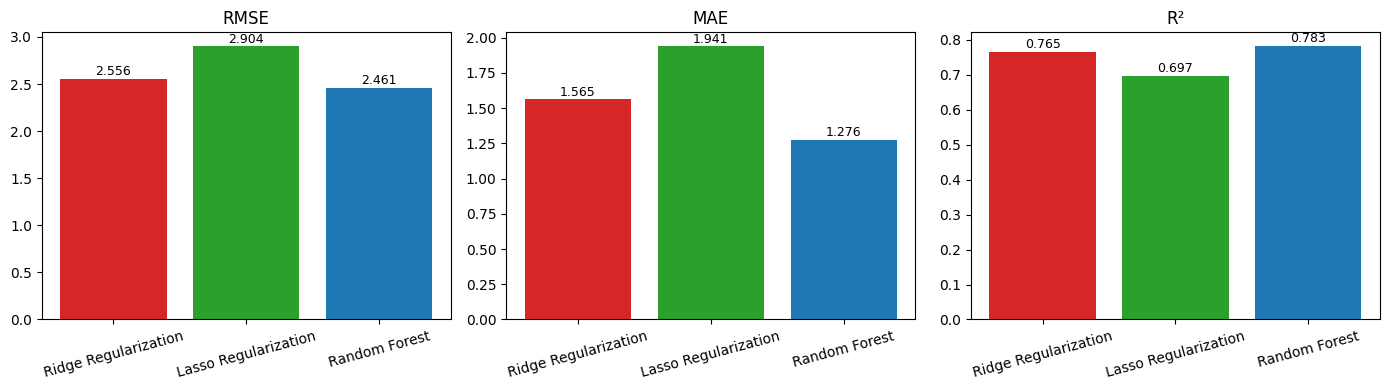
\includegraphics[width=\linewidth]{figs/f4.png}
\caption{Comparación de RMSE, MAE y $R^2$ para Ridge, Lasso y Random Forest (Linear Regression excluida).}\label{fig:reg}
\end{figure}

\paragraph{Importancia de variables}
Las variables más determinantes coinciden entre Lasso y Random Forest: \code{nota\_media\_1sem} y \code{asignaturas\_1sem\_aprobadas}. Lasso reduce todos los demás coeficientes a cero, lo que indica que, con este nivel de regularización, el resto de variables aporta poco una vez controladas esas dos. Random Forest, que mide la reducción de impureza asociada a cada variable, llega a la misma conclusión. Ridge, al no anular coeficientes, reparte el peso entre cientos de variables categóricas, por lo que su top 20 está dominado por categorías con pocas instancias (p.\,ej., \code{nacionalidad\_mozambiquena} o \code{cualificacion\_padre\_curso\_tecnico\_profesional}) que el modelo no penaliza lo suficiente.

\section{Aprendizaje No Supervisado}

El objetivo de esta sección es descubrir perfiles de estudiantes sin usar la etiqueta objetivo, combinando PCA para reducir la dimensionalidad con K-Means para agrupar a los estudiantes.

\paragraph{Selección de variables y reducción de dimensionalidad}
Se emplean únicamente las 19 variables numéricas del conjunto de datos (de ambos semestres). Las variables categóricas se excluyen deliberadamente: tras el one-hot encoding generarían cientos de columnas binarias que introducen ruido en las distancias euclídeas de K-Means. Se aplica PCA sobre los datos escalados (media 0, desviación típica 1), seleccionando 8 componentes principales que explican un 83,2\,\% de la varianza, lo que preserva la mayor parte de la información reduciendo el ruido.

\begin{table}[H]
\centering
\caption{Varianza acumulada según el número de componentes principales.}
\begin{tabular}{cc}
\toprule
Componentes & Varianza explicada\\
\midrule
3 & 50\,\%\\ 6 & 70\,\%\\ 8 & 80\,\%\\ 10 & 90\,\%\\ 13 & 95\,\%\\ 16 & 99\,\%\\ 19 & 99,9\,\%\\
\bottomrule
\end{tabular}
\end{table}

\paragraph{Elección del número de clusters}
Se evalúan dos métricas sobre el espacio reducido de 8 componentes: la inercia (método del codo), que sitúa el codo en $k=3$, y el Silhouette score, cuyo máximo se obtiene en $k=2$ (0,490; con $k=3$ es 0,367). Se trabaja con ambos valores para comparar resultados. $k=3$ resulta especialmente relevante por coincidir con el número de clases reales de la variable objetivo.

\begin{figure}[!htb]
\centering
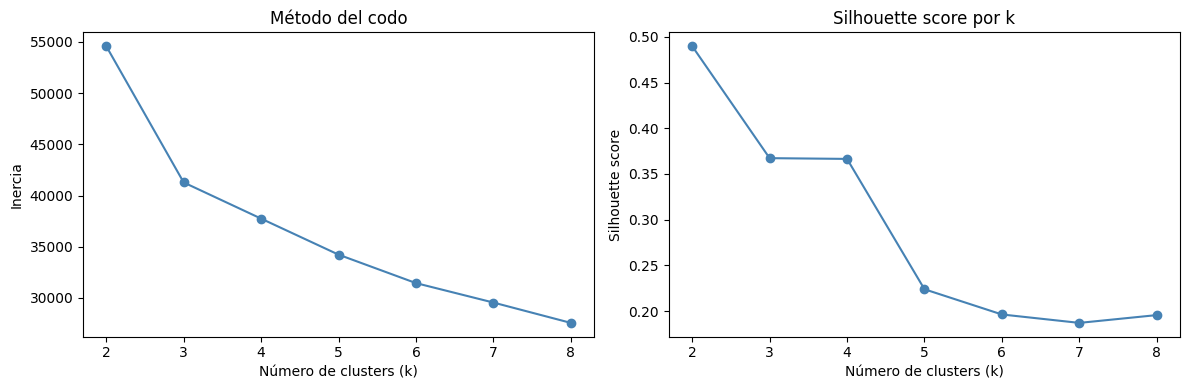
\includegraphics[width=0.85\linewidth]{figs/f5.png}
\caption{Método del codo (izquierda) y Silhouette score (derecha) para $k\in[2,8]$.}
\end{figure}

\paragraph{Interpretación de los clusters ($k=3$)}

\begin{table}[H]
\centering
\caption{Perfil medio por cluster (variables seleccionadas).}
\begin{tabular}{lccc}
\toprule
Variable & Cluster 0 & Cluster 1 & Cluster 2\\
\midrule
Nota media 1.\textsuperscript{er} sem. & 1,80 & 12,72 & 12,67\\
Asignaturas aprobadas 1.\textsuperscript{er} sem. & 0,33 & 5,25 & 11,83\\
Nota media 2.\textsuperscript{o} sem. & 0,56 & 12,49 & 12,69\\
Asignaturas aprobadas 2.\textsuperscript{o} sem. & 0,08 & 5,09 & 10,11\\
Edad al matricularse & 25,99 & 22,13 & 28,72\\
\bottomrule
\end{tabular}
\end{table}

\begin{itemize}
\item \textbf{Cluster 0 -- Bajo rendimiento} (842 estudiantes): notas prácticamente nulas y casi ninguna asignatura aprobada; corresponde mayoritariamente a estudiantes que abandonan (82,2\,\%).
\item \textbf{Cluster 1 -- Rendimiento medio} (3.316): notas en torno a 12,7 puntos y 5--6 asignaturas aprobadas por semestre; mezcla de matriculados (20,6\,\%) y graduados (59,2\,\%).
\item \textbf{Cluster 2 -- Alto número de asignaturas} (266): nota similar al cluster 1 pero con el doble de asignaturas aprobadas, mayor edad media (28,7 años) y muchas asignaturas convalidadas; predominan los graduados (64,3\,\%).
\end{itemize}

\paragraph{Contraste con la etiqueta real}

\begin{table}[H]
\centering
\caption{Distribución de la variable objetivo real por cluster ($k=3$).}
\begin{tabular}{cccc}
\toprule
Cluster & Abandono & Graduado & Matriculado\\
\midrule
0 & 82,2\,\% & 9,0\,\% & 8,8\,\%\\
1 & 20,2\,\% & 59,2\,\% & 20,6\,\%\\
2 & 22,2\,\% & 64,3\,\% & 13,5\,\%\\
\bottomrule
\end{tabular}
\end{table}

Sin haber utilizado la etiqueta objetivo en el aprendizaje, el cluster 0 agrupa estudiantes con un 82,2\,\% de abandono (692 de 842), aunque recoge algo menos de la mitad (48,7\,\%) de todos los abandonos. Esto indica que un rendimiento casi nulo se asocia fuertemente con el abandono. Los clusters 1 y 2 tienen composiciones parecidas y se distinguen sobre todo por la edad y las convalidaciones, más que por el desenlace. Cabe señalar que K-Means utiliza también variables del segundo semestre.

\begin{figure}[!htb]
\centering
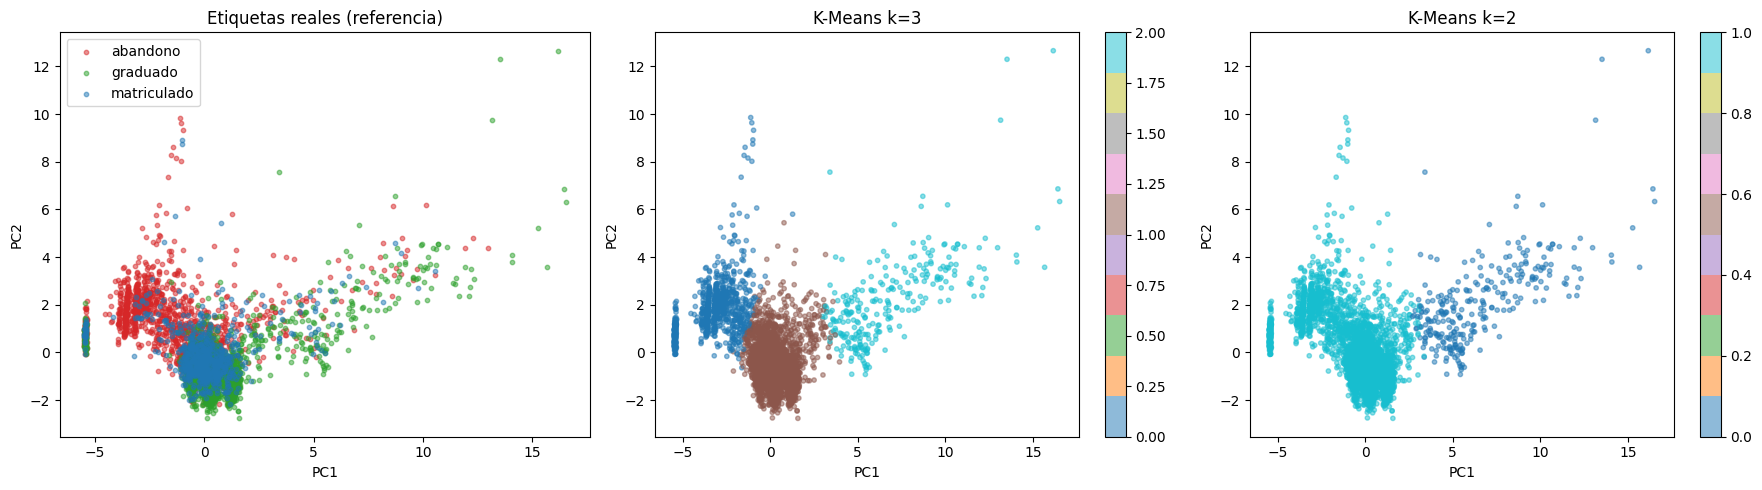
\includegraphics[width=\linewidth]{figs/f6.png}
\caption{Proyección sobre PC1--PC2: etiquetas reales (izquierda), K-Means $k=3$ (centro) y $k=2$ (derecha). En esta proyección (45\,\% de la varianza) los clusters forman regiones bien delimitadas, mientras que las clases reales se solapan, sobre todo Graduado y Matriculado.}
\end{figure}

\section{Interpretación crítica de los resultados}

\paragraph{El rendimiento académico como predictor dominante}
El hallazgo más relevante del estudio es que el rendimiento académico (principalmente asignaturas aprobadas y nota media) es el predictor dominante del éxito o fracaso académico. Este patrón aparece en los tres tipos de modelos:
\begin{itemize}
\item En \textbf{clasificación}, \code{asignaturas\_2sem\_aprobadas} es la variable más importante en los tres modelos, y las asignaturas aprobadas del primer semestre figuran entre las tres primeras en todos ellos.
\item En \textbf{regresión}, Lasso selecciona exclusivamente \code{nota\_media\_1sem} y \code{asignaturas\_1sem\_aprobadas}; Random Forest las prioriza con gran diferencia.
\item En \textbf{clustering}, K-Means, sin acceder a la etiqueta objetivo, forma un cluster de bajo rendimiento con un 82,2\,\% de abandono.
\end{itemize}

\paragraph{Contexto socioeconómico}
Las variables familiares (ocupación y cualificación de los padres, nacionalidad) no contribuyen de forma relevante una vez controlado el rendimiento académico. Su aparición en el top 20 de Ridge se explica probablemente por propiedades del modelo: al no anular coeficientes, reparte el peso entre todas las variables y asigna pesos elevados a categorías muy poco frecuentes (p.\,ej., hay solo 2 estudiantes de nacionalidad mozambiqueña). Que el contexto socioeconómico no aparezca como predictor relevante no significa que no influya en el rendimiento de un estudiante universitario; sin embargo, una vez se tienen los resultados académicos, estos prevalecen sobre cualquier otro tipo de variable.

\paragraph{Clasificación vs. regresión}
Ambos modelos abordan el mismo fenómeno de diferente forma. La clasificación determina si un estudiante acabará graduándose, abandonando o continuando matriculado, la pregunta con mayor valor para la institución. La regresión estima la nota concreta que obtendrá en el segundo semestre a partir de variables del primero y del contexto del estudiante, lo que la convierte en una herramienta útil para anticipar el rendimiento futuro antes de que ocurra.

El F1-macro de 0,72 alcanzado en clasificación indica que los modelos capturan patrones reales, pero con margen de mejora. La clase Matriculado concentra los errores de predicción, lo cual tiene cierto sentido: al tratarse de estudiantes que aún no han terminado su titulación, su desenlace final es desconocido.

\paragraph{El clustering como contraste}
Que K-Means, sin usar la etiqueta, aísle un grupo de rendimiento casi nulo con un 82,2\,\% de abandono apoya que el rendimiento académico es el principal eje de variación de los datos. La correspondencia con las tres clases reales es, en cambio, parcial: los clusters 1 y 2 no separan graduados de matriculados, sino perfiles de edad y convalidaciones.

\section{Conclusiones finales y posibles limitaciones del estudio}

\paragraph{Conclusiones principales}
\begin{enumerate}
\item \textbf{Rendimiento académico:} la nota media y las asignaturas aprobadas son los predictores más potentes del resultado académico, de forma consistente en los tres tipos de modelo. En regresión, las variables del primer semestre, junto con las de contexto, permiten estimar la nota del segundo ($R^2\approx0{,}78$).
\item \textbf{Modelos lineales vs. no lineales:} en clasificación, la regresión logística obtiene el mejor F1-macro (0,72), por delante de Gradient Boosting (0,69) y Random Forest (0,68); en regresión, Random Forest logra el mejor ajuste ($R^2\approx0{,}78$), seguido de Ridge (0,765). En regresión, la ventaja del modelo no lineal sobre Ridge es pequeña, y Lasso ofrece una selección automática de variables útil para la toma de decisiones, al identificar las que concentran la información relevante.
\item \textbf{Contexto socioeconómico:} las variables familiares no son seleccionadas por Lasso en regresión y tienen importancias marginales en los árboles. Esto no implica que el origen socioeconómico sea irrelevante en el acceso o la preparación previa, pero sí que no mejora la predicción una vez conocido el rendimiento académico.
\item \textbf{Estructura de los datos:} el clustering aísla un grupo de bajo rendimiento muy asociado al abandono; los otros grupos se distinguen más por edad y convalidaciones que por su desenlace.
\end{enumerate}

\paragraph{Limitaciones del estudio}
\begin{enumerate}
\item \textbf{Representatividad de los datos.} El conjunto proviene de una única institución. Los resultados pueden no generalizarse a sistemas con culturas académicas o perfiles de alumnado distintos.
\item \textbf{Variable objetivo basada en el estado final.} La clase Matriculado agrupa estudiantes cuyo destino es aún desconocido, introduciendo ruido en los modelos y deflactando probablemente las métricas reales.
\item \textbf{Desbalance de clases.} Las tres clases no están uniformemente distribuidas, lo que puede sesgar los resultados hacia las clases mayoritarias pese al uso de métricas ajustadas (F1-macro).
\item \textbf{Evaluación con una única partición.} No se emplea validación cruzada ni ajuste de hiperparámetros (se usan valores por defecto y $\alpha=1$ en Ridge y Lasso), por lo que las diferencias pequeñas entre modelos no deben sobreinterpretarse. Además, cerca del 20\,\% de los valores de \code{nota\_media\_2sem} son exactamente 0, lo que genera colas de error en la regresión.
\item \textbf{Uso como alerta temprana.} El clasificador emplea variables del segundo semestre, por lo que no es un sistema de alerta temprana; para ese fin habría que entrenar con la información disponible en el momento de la intervención.
\item \textbf{Interpretabilidad causal limitada.} La correlación entre el rendimiento y el resultado final no implica causalidad: ambos podrían estar mediados por factores no observados como la motivación o las circunstancias personales. Faltan variables como horas de asistencia o de estudio que podrían ayudar a perfilar mejor los resultados.
\end{enumerate}

\section{Bibliografía}
\begin{itemize}[leftmargin=1.2em,itemsep=3pt]
\small
\item Realinho, V., Vieira Martins, M., Machado, J. y Baptista, L. (2021). \emph{Predict Students' Dropout and Academic Success}. UCI Machine Learning Repository. \url{https://doi.org/10.24432/C5MC89}
\item Realinho, V., Machado, J., Baptista, L. y Vieira Martins, M. (2022). Predicting Student Dropout and Academic Success. \emph{Data}, 7(11), 146. \url{https://doi.org/10.3390/data7110146}
\item Pedregosa, F. et al. (2011). Scikit-learn: Machine Learning in Python. \emph{Journal of Machine Learning Research}, 12, 2825--2830.
\item Scikit-learn developers (2024). scikit-learn 1.4 Documentation. \url{https://scikit-learn.org/stable/}
\item Scikit-learn developers (2024). sklearn.ensemble.RandomForestClassifier. \url{https://scikit-learn.org/stable/modules/generated/sklearn.ensemble.RandomForestClassifier.html}
\item Scikit-learn developers (2024). sklearn.ensemble.GradientBoostingClassifier. \url{https://scikit-learn.org/stable/modules/generated/sklearn.ensemble.GradientBoostingClassifier.html}
\item Scikit-learn developers (2024). sklearn.linear\_model.Lasso. \url{https://scikit-learn.org/stable/modules/generated/sklearn.linear_model.Lasso.html}
\item Scikit-learn developers (2024). sklearn.linear\_model.Ridge. \url{https://scikit-learn.org/stable/modules/generated/sklearn.linear_model.Ridge.html}
\item Scikit-learn developers (2024). sklearn.cluster.KMeans. \url{https://scikit-learn.org/stable/modules/generated/sklearn.cluster.KMeans.html}
\end{itemize}

\end{document}
